\documentclass{article}
\usepackage{icml2021} % You need to have the ICML 2022 style file
\usepackage{graphicx}
\usepackage{amsmath}
\usepackage{hyperref}
\usepackage{graphicx} %package to manage images
\graphicspath{ {images/} }

\title{Review of "PESNet: Ab-Initio Potential Energy Surfaces by Pairing GNNs with Neural Wave Functions"}
\author{\textbf{Philip Hierhager}\\Department of Informatics\\Technical University of Munich, Germany\\
\texttt{philip.hierhager@tum.de}
}
\date{20.08.2024}

\begin{document}

\maketitle

\begin{abstract}
    The report provides a critical review of the paper "PESNet: Ab-Initio Potential Energy Surfaces by Pairing GNNs with Neural Wave Functions" by Nicholas Gao and Stephan Günnemann. In it, the authors describe a new approach combining Graph Neural Networks (GNNs) and neural wave functions to solve the Schrödinger equation for multiple molecular geometries simultaneously, significantly reducing computational costs. This review summarizes the main contributions, strengths, limitations, and potential future research directions based on the findings of the paper.
\end{abstract}

\section{Introduction}
The paper "PESNet: Ab-Initio Potential Energy Surfaces by Pairing GNNs with Neural Wave Functions" addresses the computational challenges in solving the Schrödinger equation for multiple molecular geometries with neural networks. Using neural wave functions as a represantion of the quantum wave function still requires separate self-supervised trainings with the Variational Monte Carlo (VMC) framework for each geometry, leading to high computational costs. Orthogonal research has been conducted to reformulate the eigenvalue problem of solving the Schrödinger equation as a supervised regression task. It models the system with graph neural networks (GNN) and takes features like position and charge of the nuclei and regresses on its energy. The labels come from classical simulation like Coupled Clusters (CC) and Density Function Theory(DFT). However, as graph neural networks became very performant in the task, the error of the simulated data to the real-world data is larger than the error of the neural network. The authors propose PESNet, which leverages GNNs to parameterize a neural wave function, allowing simultaneous resolution of the Schrödinger equation for multiple geometries. The significance of this approach lies in its ability to capture the potential energy surfaces (PES) more efficiently and accurately, which is crucial for understanding molecular interactions and reactions. It combines the strengths of GNNs and neural wave functions approach to model the quantum state of molecular systems.

\section{Method Summary}
The proposed PESNet architecture integrates a MetaGNN with a wave function model (WFModel) to generate parameters for multiple molecular geometries. The MetaGNN processes the nuclei coordinates and charges, outputting parameters that adapt the WFModel for specific geometries. This method captures continuous subsets of the potential energy surface in a single training pass, enhancing efficiency. Key components of the approach include:
\begin{itemize}
    \item \textbf{Variational Monte Carlo (VMC) Framework}: The use of VMC allows for an efficient and flexible approach to approximate the ground-state wave functions by minimizing the energy expectation value. This is used to train the neural wave function model.
    \item \textbf{Equivariant Coordinate System}: To handle physical symmetries and ensure the wave function respects the symmetries of the molecular system, an equivariant coordinate system is introduced.
    \item \textbf{MetaGNN Architecture}: The MetaGNN encodes the molecular geometry information and produces parameters that are used by the WFModel. This includes various layers such as message-passing layers that capture interactions between atoms.
    \item \textbf{Wave Function Model (WFModel)}: The WFModel is responsible for generating the wave function given the parameters from MetaGNN. It includes neural network components designed to approximate the complex quantum state of the system. They use FermiNet as a basis for the model and edit it to be more efficient and accurate. This is done by introducing an invariance to nuclei reindexing by summation instead of concetanation and by decreasing the solution space using the Equivariant Coordinate System. The model is trained using the VMC framework.
\end{itemize}
The combination of these components allows PESNet to efficiently and accurately model the potential energy surfaces for a variety of molecular geometries. The interactions between the MetaGNN and WFModel are depicted in figure \ref{fig:schematic}.

\begin{figure}[h]
    \centering
    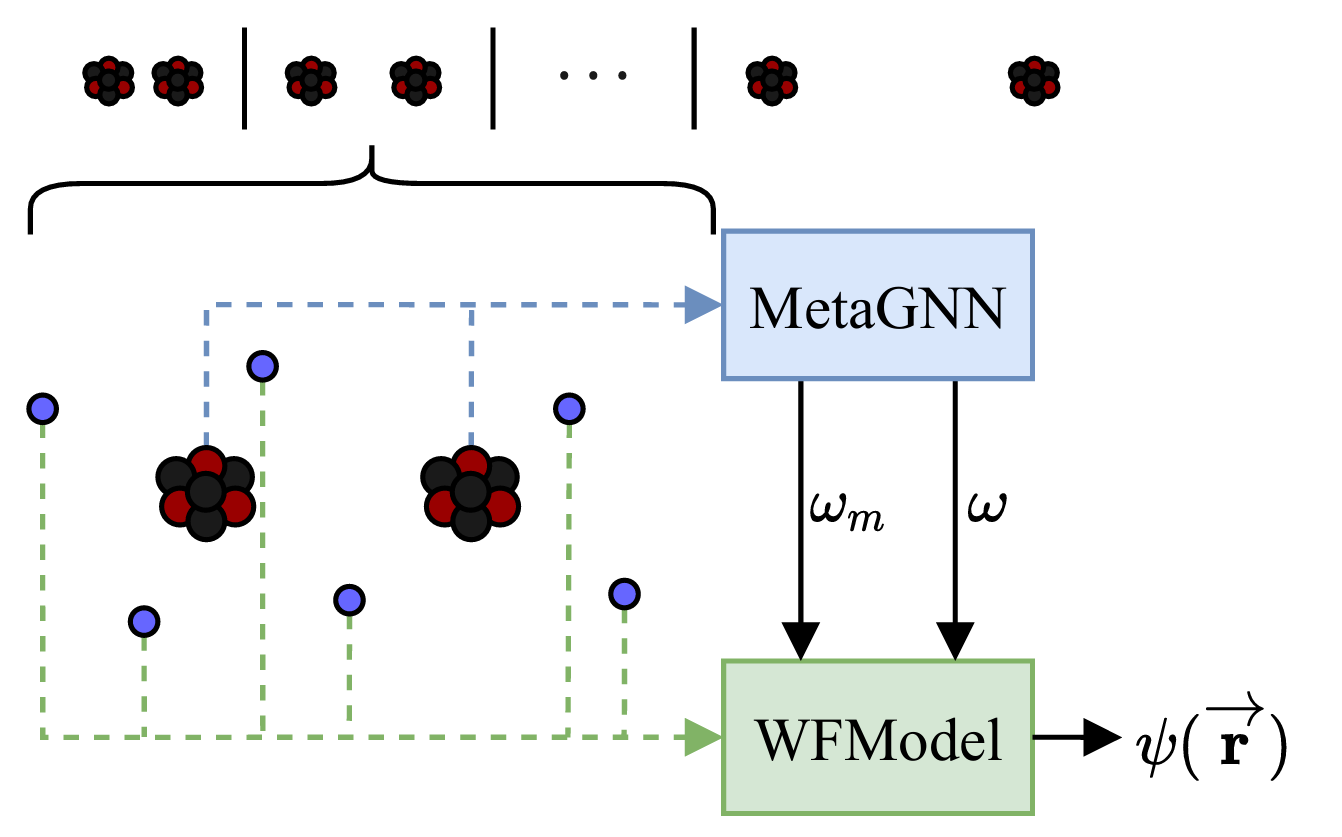
\includegraphics[width=0.5\textwidth]{schematic_pesnet.png}
    \caption{Schematic of PESNet. For every molecular structure, the MetaGNN processes the charges and distances and parametrizes the WFModel. Given these, the WFModel evaluates the electronic wave function. (Image taken from the paper)}
    \label{fig:schematic}
\end{figure}

\section{Relation to Literature}
The paper builds on previous works that employ neural networks for quantum mechanical calculations. The authors reference various surrogate models and neural wave function methods, highlighting the limitations of existing approaches and positioning PESNet as a significant advancement.

\subsection{Comparison with Traditional Surrogate Models}
Traditional surrogate models require labels from classical quantum mechanical simulations leading to errorenous data. Several works are summarized here.
\begin{itemize}
    \item \textbf{SchNet}: In "SchNet: A Continuous-filter Convolutional Neural Network for Modeling Quantum Interactions"~\cite{schuttSchNetDeepLearning2018}, the authors propose SchNet, a deep learning model designed to predict molecular properties. It uses continuous-filter convolutional layers to handle molecular graphs, capturing both geometric and chemical information effectively. It was not used in the PESNet paper.
    \item \textbf{HiGNN}: In "Hierarchical Graph Neural Networks for 3D Molecular Structure Prediction"~\citep{yangAnalyzingLearnedMolecular2019}, the authors introduce a hierarchical approach to graph neural networks for predicting 3D molecular structures. The proposed model combines local and global graph information, enabling it to capture both fine-grained atomic interactions and broader structural patterns. This approach significantly enhances the accuracy of molecular property predictions and the understanding of molecular dynamics. It was not directly used in the PESNet paper.
    \item \textbf{DimeNet}: In "Directional Message Passing for Molecular Graphs"~\citep{klicperaDirectionalMessagePassing2019}, the authors introduce the DimeNet model, which uses directional message passing for molecular graphs. It improves upon traditional GNNs by incorporating directional information between atoms, allowing for a more accurate representation of molecular structures and better predictions of quantum mechanical properties. The angles between atoms are taken into account by using spherical Bessel functions. Together with the distances of the atoms in the molecule embedded with radial Bessel functions the message passing functions are modelled. The authors of PESNet use a revised version of DimeNet as their MetaGNN leaving out the cutoff and envelope as their WFModel already takes care of only modelling wave functions that decay to zero far away from the molecule. Like DimeNet it encodes the molecular geometry information with charges, distances of the nuclei and angles between them. The model is then used to generate parameters for the WFModel.
    \item \textbf{Other recent work}: More recent work focuses on how to incorporate calculations from quantum chemistry to make the ground truth labels more accurate. This includes models like QDF~\citep{tsubakiQuantumDeepField2020}, EANN~\citep{zhangEmbeddedAtomNeural2019}, UNiTE~\citep{qiaoUNiTEUnitaryNbody2021}, $\Delta$-ML models~\citep{wengertDataefficientMachineLearning2021}. The main problem however still persists: All of the surrogate models focus on solving quantum-mechanical calculations from simulated and not real ground truth data. PESNet aims for the exact calculations from first-principles using only inductive biases and the Schrödinger equation itself to solve it.
\end{itemize}


\subsection{Advances over Neural Wave Function Methods}
Physicists normally used traditional self-consistent field methods such as Hartree-Fock, Density Functional Theory (DFT) or Coupled Cluster (CC) to solve the Schrödinger equation by first simplifying the representation of the quantum system and then employing a specific solver. However, these methods are computationally expensive and often require significant approximations. In combination with the VMC framework, neural wave functions have been proposed as a mean to represent the wave function of quantum system in a compressed but yet accurate way. The first work was "Solving the Quantum Many-Body Problem with Artificial Neural Networks"~\citep{carleoSolvingQuantumManyBody2017} where they used neural networks to create a variational represantion of quantum states. The first models that dealt with larger systems were FermiNet~\citep{pfauInitioSolutionManyelectron2020} and PauliNet~\citep{hermannDeepneuralnetworkSolutionElectronic2020}. Both models were able to solve the Schrödinger equation for larger systems and with higher accuracy than traditional methods. On top of that, recently PsiFormer~\citep{vonglehn2023selfattentionansatzabinitioquantum} which is a transformer-based model. All models are trained with the VMC framework, but others like the Diffusion Monte Carlo can also be used like in this paper with FermiNet~\cite{wilsonSimulationsStateoftheartFermionic2021} or in the PauliNet paperw where they compare DMC and VMC.
\begin{itemize}
    \item \textbf{FermiNet}: FermiNet is a neural network model that approximates the many-body wave function of a quantum system. It uses a graph neural network architecture that respects the antisymmetry of the wave function, allowing it to model the quantum state of many-electron systems accurately. It uses Slater Determinants for the antisymmetry and the Kronecker-factored approximate curvature (KFAC) as an approximation to natural gradient descent. It uses a permutation-invariant architecture to handle the indistinguishability of electrons and is able to model the cusp conditions by using nondifferentiable input features. FermiNet is used as the basis for the WFModel in the PESNet paper.
    \item \textbf{PauliNet}: PauliNet is another neural network model designed to solve the electronic Schrödinger equation for many-electron systems. It uses a deep neural network architecture that respects the Pauli exclusion principle, ensuring that the wave function is antisymmetric with respect to the electron coordinates. This model has been shown to achieve high accuracy in predicting quantum mechanical properties of molecular systems. As FermiNet it uses the slater determinant so that the wave function is antisymmetric. On top of that, PauliNet integrates physical constraints, such as the cusp conditions - the behavior of the wavefunction when electrons approach each other or the nuclei - directly into the neural network by using Jastrow factors. Thus, PauliNet has a stronger inductive bias than FermiNet when modelling the wave function.
    \item \textbf{PsiFormer}: PsiFormer is a transformer-based model that leverages self-attention mechanisms to model the quantum wave function of many-electron systems. It uses a transformer architecture to capture long-range interactions and dependencies within the molecular system. As the self-attention layer is permutation equivariant, the model becomes invariant to the ordering of atoms and molecules. Like PauliNet and FermiNet it uses the slater determinant to model the antisymmetric total wavefunction. The authors of the PsiFormer paper claim that their model is more efficient and accurate than FermiNet and PauliNet.
\end{itemize}

\subsection{Other works combining meta models with neural wave functions}
\begin{itemize}
    \item \textbf{DeepErwin}: The model DeepErwin introduced in the paper "Gold-standard solutions to the Schrödinger equation using deep learning: How much physics do we need?"~\cite{gerardDeepErwin} combines the FermiNet model with the SchNet model. Furthermore, it uses a equivariant coordinate system like in PESNet, however local, centered on every nucleus. They also propose a new way of enveloping the wave function, giving it less freedom for faster convergence, lower final energies, and lower variance.
\end{itemize}

\section{Strengths}
PESNet demonstrates several strengths, including:
\begin{itemize}
    \item \textbf{Efficiency}: By handling multiple geometries simultaneously, PESNet reduces the computational cost significantly compared to traditional methods that train separately for each geometry. On large molecules the speedup can be up to 40 times as it can be seen in the table below \ref{fig:gpu_times}.
    \item \textbf{Accuracy}: The use of GNNs and neural wave functions enables PESNet to model the potential energy surfaces with high accuracy, on par with FermiNet which is trained for every geometry as can be seen in figure \ref{fig:comparison}.
    \item \textbf{Incorporation of Physical Symmetries}: The use of an equivariant coordinate system ensures that the model respects the symmetries of the molecular systems, leading to more physically accurate representations and more efficient training.
    \item \textbf{Scalability}: The architecture of PESNet is designed to be scalable, allowing it to handle larger and more complex molecular systems effectively. PESNet is able to handle larger molecules than other meta-learning approaches as DeepErwin as it can be seen in the table below \ref{fig:gpu_times}.
\end{itemize}

\begin{figure}[h]
    \centering
    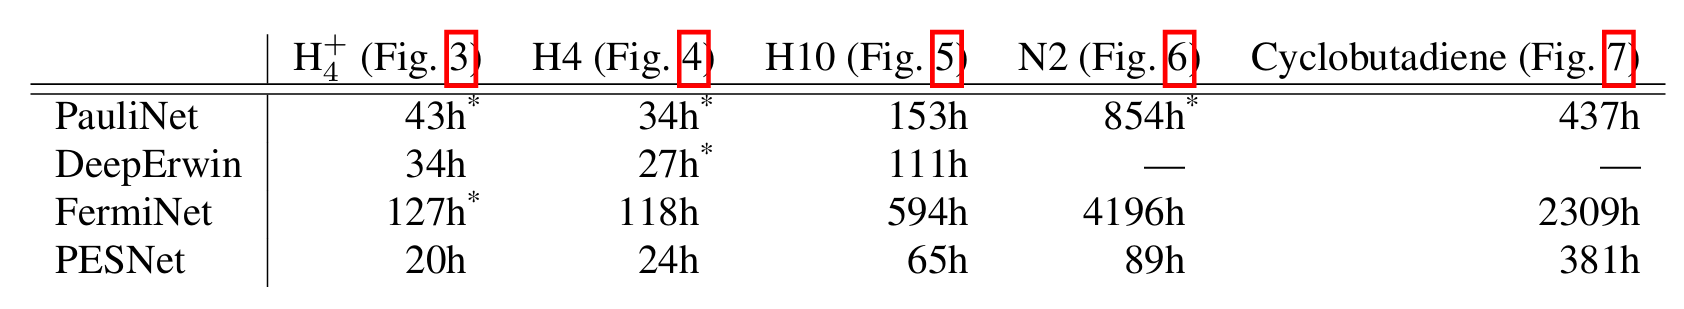
\includegraphics[width=0.5\textwidth]{table_gpu_times.png}
    \caption{Total GPU (A100) hours to train all models of the respective figures. PESNet is up to 40 times faster than FermiNet and in all benchmarks faster than DeepErwin. It also more scalable as DeepErwin is not able to handle the largest molecules. (Image taken from the paper)}
    \label{fig:gpu_times}
\end{figure}

\begin{figure}[h]
    \centering
    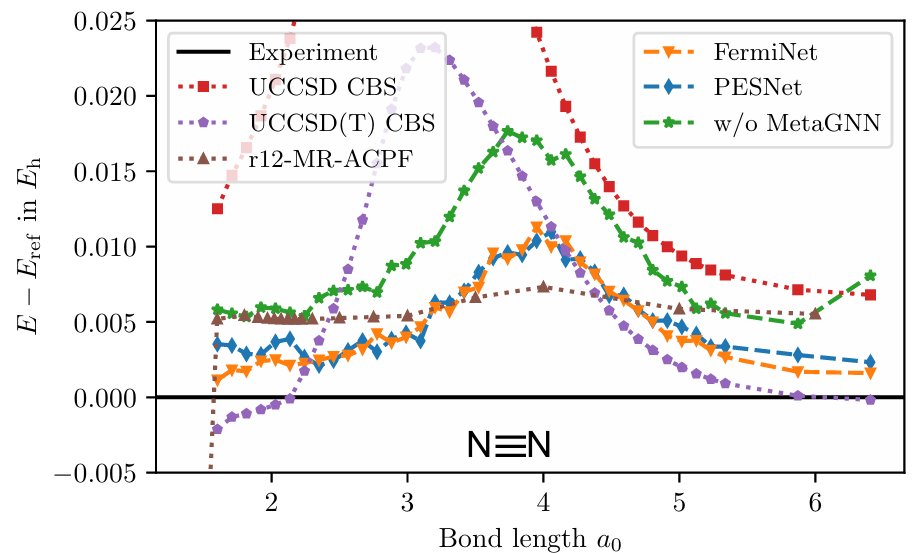
\includegraphics[width=0.5\textwidth]{FermiNet_PesNet_comparison}
    \caption{Potential energy surface scan of the
        nitrogen molecule. PESNet yields very similar energies than FermiNet. Without the MetaGNN the accuracy drops significantly. (Image taken from the paper)}
    \label{fig:comparison}
\end{figure}

\section{Limitations}
Despite its strengths, PESNet has some limitations:
\begin{itemize}
    \item \textbf{Scalability to Extremely Large Systems}: While PESNet is scalable, its performance and accuracy is unclear on extremely large molecular systems with many atoms.
    \item \textbf{Validation Range}: The paper demonstrates results on a limited range of molecular geometries and configurations. More extensive validation across a broader set of molecules would be beneficial.
\end{itemize}


\section{Challenges and Future Research Direction}
There are several challenges of the paper that could be addressed in future work:
\begin{itemize}
    \item \textbf{Assumptions in Model Training}: The model assumes that the chosen training configurations are representative of the entire potential energy surface, which may not always be the case in complex systems where VMC needs special sampling methods. In complex molecular systems, the potential energy surface can have many local minima, saddle points, and diverse regions.  If the training configurations do not adequately represent the entire potential energy surface, the model may not perform well in regions of the PES that were underrepresented or not sampled during training.
    \item \textbf{Interpretability}: Neural networks, including PESNet, often suffer from interpretability issues, making it challenging to understand the underlying reasons for certain predictions or errors. This can be an issue when actually using the model in practice in drug desing for example, as it is important to understand why the model makes certain predictions.
    \item \textbf{Handling Larger Systems}: Extending PESNet to handle larger and more complex molecular systems, potentially through architectural enhancements or more efficient training methods.
    \item \textbf{Improving Symmetry Integration}: Developing more sophisticated methods to integrate physical symmetries, further improving the accuracy and robustness of the model.
    \item \textbf{Robust Training Methods}: Exploring alternative training methods and frameworks to enhance the generalizability and robustness of PESNet. This also includes the evaluation fo different optimizers and different sampling methods.
    \item \textbf{Expanding Validation}: Conducting more extensive validation studies across a broader range of molecules and configurations to establish the generalizability of PESNet.
\end{itemize}

\section{Conference Review Perspective}
As ICLR reviewers of the paper confirmed by putting it into the ICLR Spotlight position, the paper is very innovative, combining two state-of-the-art orthogonal research directions to solve a very hard problem in quantum chemistry. The paper is well-written and clearly presents the methodology, results, and implications of the research. It also is clearly structured, so that even people without knowledge in chemistry can understand the subject. Furthermore, the figures helped a lot to get an insight into the model and the research. As an example, the figure \ref{fig:architecture} explains the whole model architecture graphically. The experimental evaluation is thorough, demonstrating the efficiency of the proposed PESNet model. Overall, the paper is a significant contribution to the field of computational quantum chemistry.

\begin{figure}[h]
    \centering
    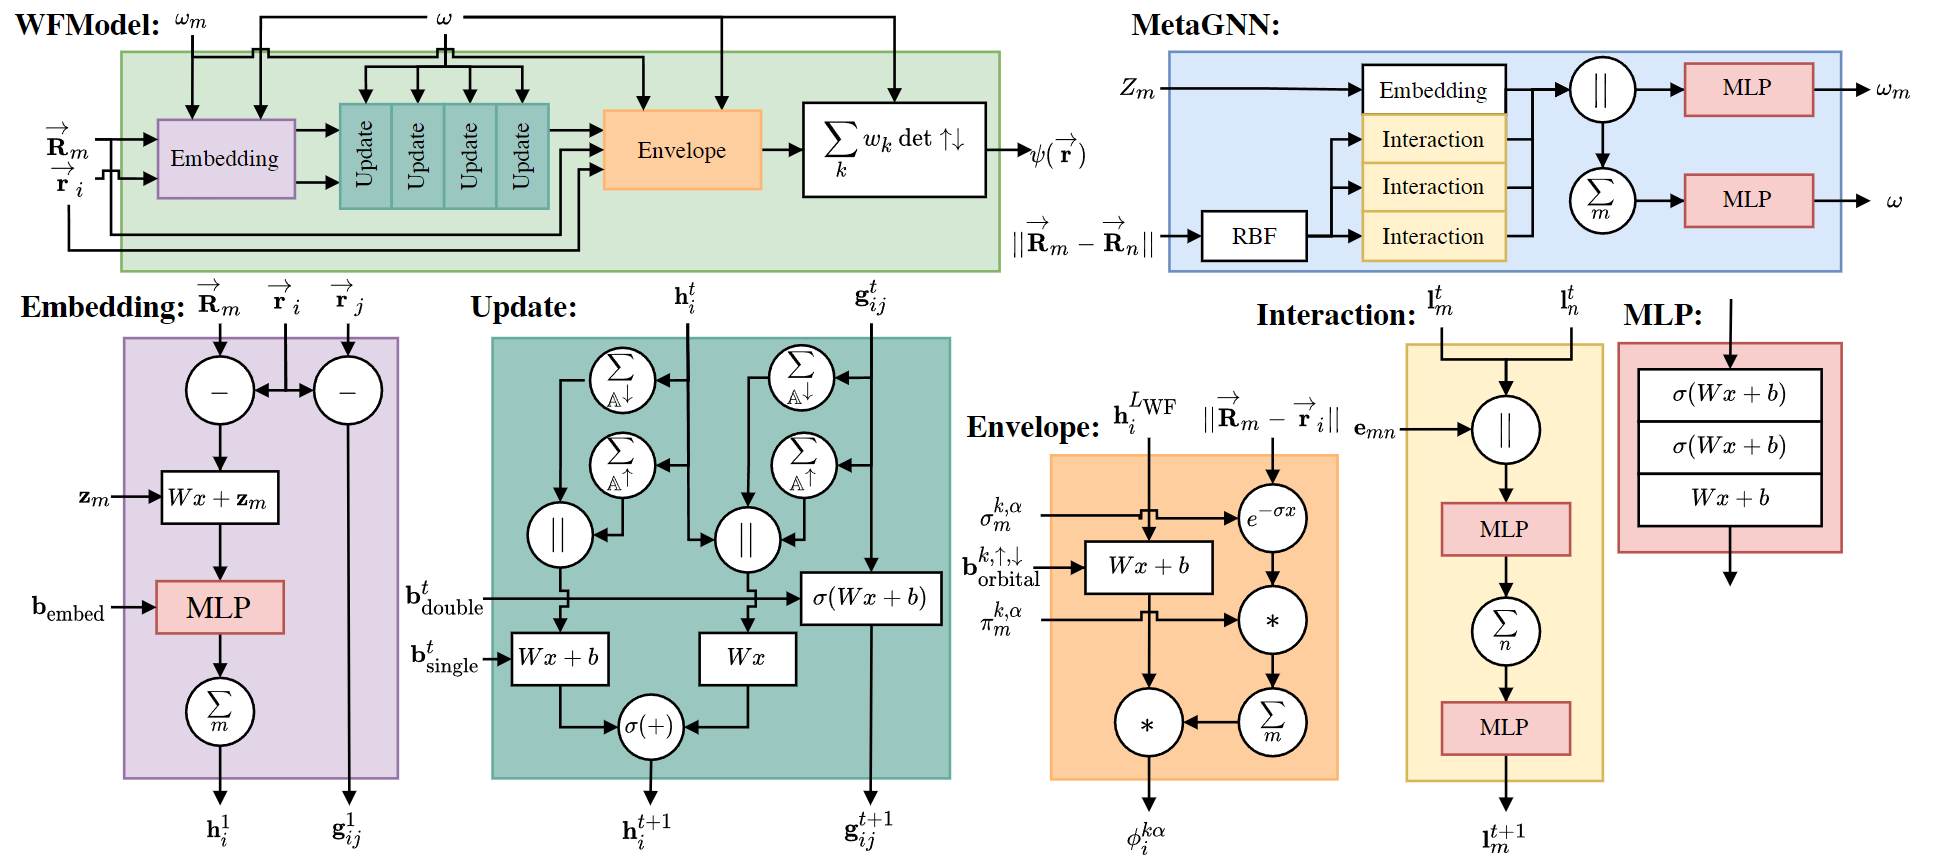
\includegraphics[width=0.5\textwidth]{architecture_.png}
    \caption{The PESNet architecture is split into two main components, the MetaGNN and the WFModel. The MetaGNN processes the molecular geometry information and generates parameters for the WFModel, which evaluates the electronic wave function. (Image taken from the paper)}
    \label{fig:architecture}
\end{figure}

\section{Extension in the Community}
PESNet influenced subsequent research. Since its introduction, there have been several extensions and new research directions:
\begin{itemize}
    \item \textbf{PESNet++}: The authors extended on their model one year later with additional features and an additional inductive bias by introducing physically-motivated restricted neural wave function models in their paper "Sampling-free Inference for Ab-Initio Potential Energy Surface Networks"~\cite{gao2023samplingfree}. It reduces energy errors by up to 74\%.
    \item \textbf{PlaNet}: In the same paper of PESNet++~\cite{gao2023samplingfree}, the authors introduced PlaNet, a sampling free model that trains a surrogate model to predict the potential energies of different geometries directly. In PESNet, the inference would yield a wave function. To get the actual potential energy from it, a Monte-Carlo method has to be used which scales quartic in the number of electrons. PlaNet is able to predict the potential energy directly from the nuclei geometries.
    \item \textbf{Weight-sharing for molecular deep neural networks}: The PESNet paper inspired the authors of the paper "Solving the electronic Schrödinger equation for multiple nuclear geometries with weight-sharing deep neural networks"~\cite{scherbela2022solving} and underlined their observation that the specific solution space in this problem can be exploited by sharing weights and thus restricting the parameter space.
    \item \textbf{Globe and Moon}: In another paper "Generalizing Neural Wave Functions with Equivariant Graph Neural Networks"~\cite{gao2023generalizing}, the authors introduced Globe and Moon, two models that generalize the neural wave function models to different molecular systems. As PESNet is only able to model the potential energy surface of one molecule, and DeepErwin still need retraining for each structure, there is a need for a model that can generalize to different molecules. Graph-learned Orbital Embeddings (Globe) reparametrizes the wave function depending on the molecular structure, so it only looks at atoms and does not consider electrons. The Molecular Orbital Network (Moon) represents the electronic wave function, but encourages local interaction by incorporating spatial message passing.
\end{itemize}

\section{Conclusion}
PESNet is a significant advancement in th computational quantum chemistry field. It addresses the high computational cost by deploying a meta model that uses self-supervision to accurately predict potential energy surfaces. Its results and innovative use of GNNs demonstrate potential for further research and application. This report has summarized the key contributions, strengths, limitations, and future directions for PESNet, providing a critical review.

\bibliographystyle{icml2021}
\bibliography{pesnet_report}

\end{document}
